\begin{Exercise}[title=Pendule sur un plan incliné avec frottement]
  On considère un pendule posé sur un plan incliné, incliné d'un angle $\alpha$ par rapport à l'horizontal. On écarte le pendule de sa position d'équilibre d'un angle $\beta_0$. Il remonte de l'autre côté d'un angle $\beta_1$.
  \begin{center}
    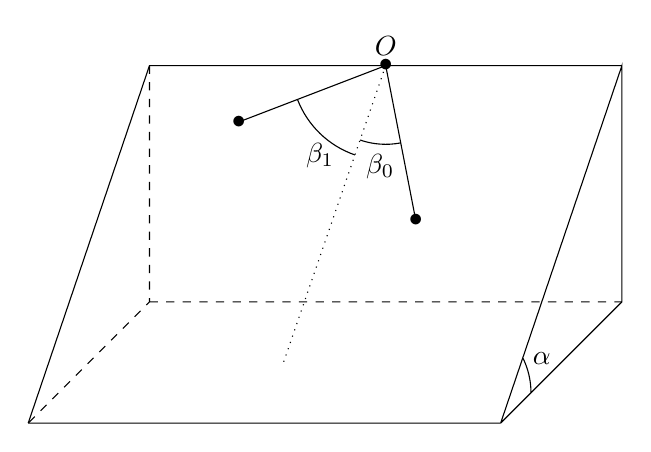
\begin{tikzpicture}
      \draw (0,0,0) -- (-6,0,0)
      (0,0,0) -- (0,0,-4) -- ++(0,3,0) -- (0,0,0)
      (0,0,-1) arc(0:26:1) node[right]{$\alpha$}
      (0,3,-4) -- ++(-6,0,0)node[midway]{$\bullet$} coordinate[midway](O) -- (-6,0,0);
      \draw[dotted] (O) node[above]{$O$} -- ++(-109:4);
      \draw (O) -- ++(-79:2)node{$\bullet$};
      \draw (O) ++(-79:1) arc(-79:-109:1) node[midway, below]{$\beta_0$};
      \draw (O) -- ++(-159:2)node{$\bullet$};
      \draw (O) ++(-159:1.2) arc(-159:-109:1.2) node[midway, below]{$\beta_1$};
      \draw[dashed] (-6,3,-4) -- (-6,0,-4)  --(-6,0,0)
      (-6,0,-4) -- ++(6,0,0);
    \end{tikzpicture}
  \end{center}
  Déterminer le coefficient de frottement $f$ en fonction de $\alpha$, $\beta_0$ et $\beta_1$.
\end{Exercise}
\begin{Answer}
  Solution
\end{Answer}
